\documentclass[fleqn,10pt]{olplainarticle}
% Use option lineno for line numbers 
\DeclareMathOperator{\sinc}{sinc}
\usepackage{subfig}

\title{Formulation of a sensing matrix for ISAR imaging of a maneuvering target with slow-time undersampling}

\author[1]{Brandon Boucher}

\keywords{ISAR, SAR, non-uniform sampling, maneuvering target, slow-time undersampling, compressed sensing}

\begin{abstract}
Inverse Synthetic Aperture Radar (ISAR) imaging enables all-weather imaging of non-cooperative targets by exploiting their rotation. However, imaging targets with non-uniform rotation or challenging trajectories induces phase errors due to inadequate motion compensation and distortion from non-uniform sampling. This is further exasperated by undersampling in slow-time, as pulses are commonly dropped during acquisition from interruption, hardware limitations or jamming. Traditional image formation techniques like Range-Doppler processing are insufficient in handling both complex target motion and slow-time undersampling, necessitating the usage of more sophisticated methods like those posed by compressed sensing. A large portion of compressed sensing algorithms including most greedy and basis pursuit algorithms are applied to linear systems, requiring a derivation of a forward operator or sensing matrix. The following document serves to derive a forward operator of a linear system describing the measurement of pulses used to form a SAR image. 
\end{abstract}

\begin{document}

\flushbottom
\maketitle
\thispagestyle{empty}



\section*{Geometry}

The crossrange resolution of ISAR images is dictated by the rotation of the target. Translational motion is seen as a nuisance, providing no value in forming the image and is typically discarded. This reduces the ISAR model to a tabletop, where the target rotates at a fixed position away from the radar. Additionally, for the purposes of specifically evaluating the effects of non-uniform sampling and slow-time undersampling, the rotation motion parameters are assumed to be known. Figure \ref{fig:geo} depicts the ISAR imaging geometry.

%\begin{figure}[ht]
%    \centering
%    \includegraphics[width=0.5\linewidth]%{isar_geometry.png}
%    \caption{Caption}
%    \label{fig:geo}
%\end{figure}

\begin{figure*}[ht]
    \centering
    \subfloat[]{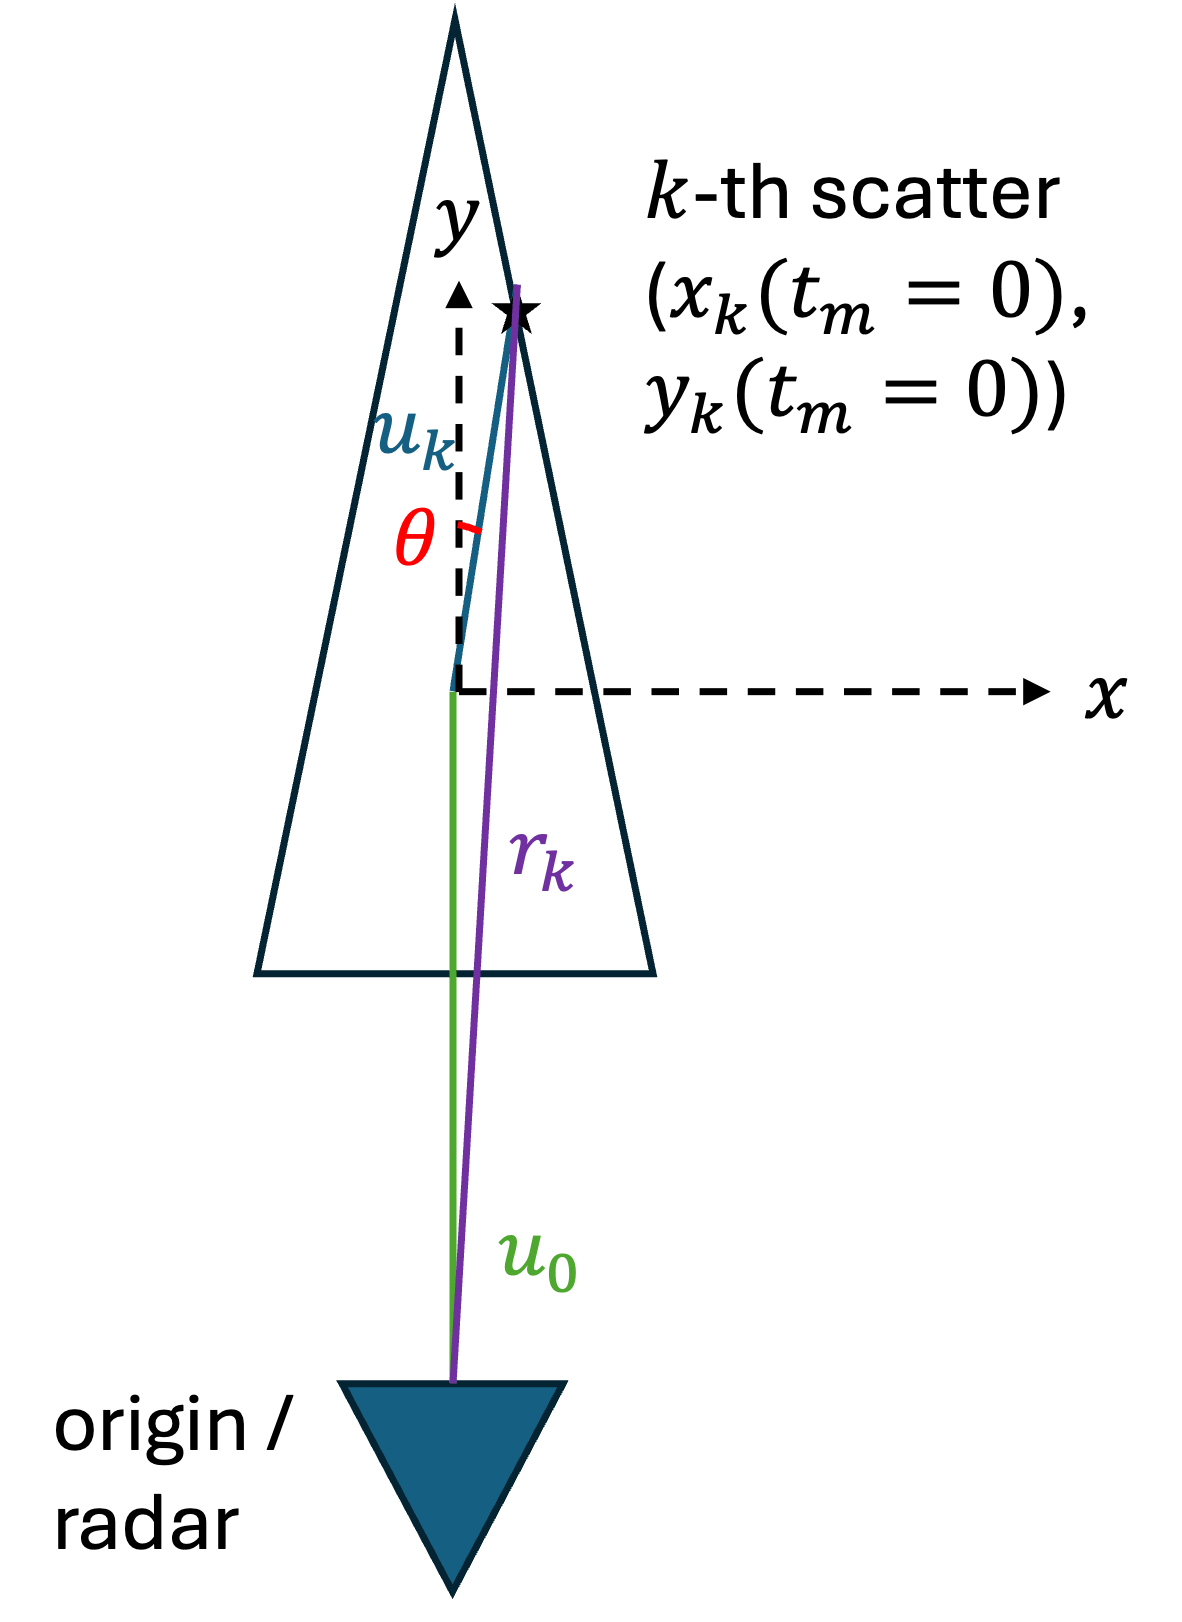
\includegraphics[width=0.3\linewidth]{isar_geo1.png}}%
    \label{fig:psf_b}
    \hfil
    \subfloat[]{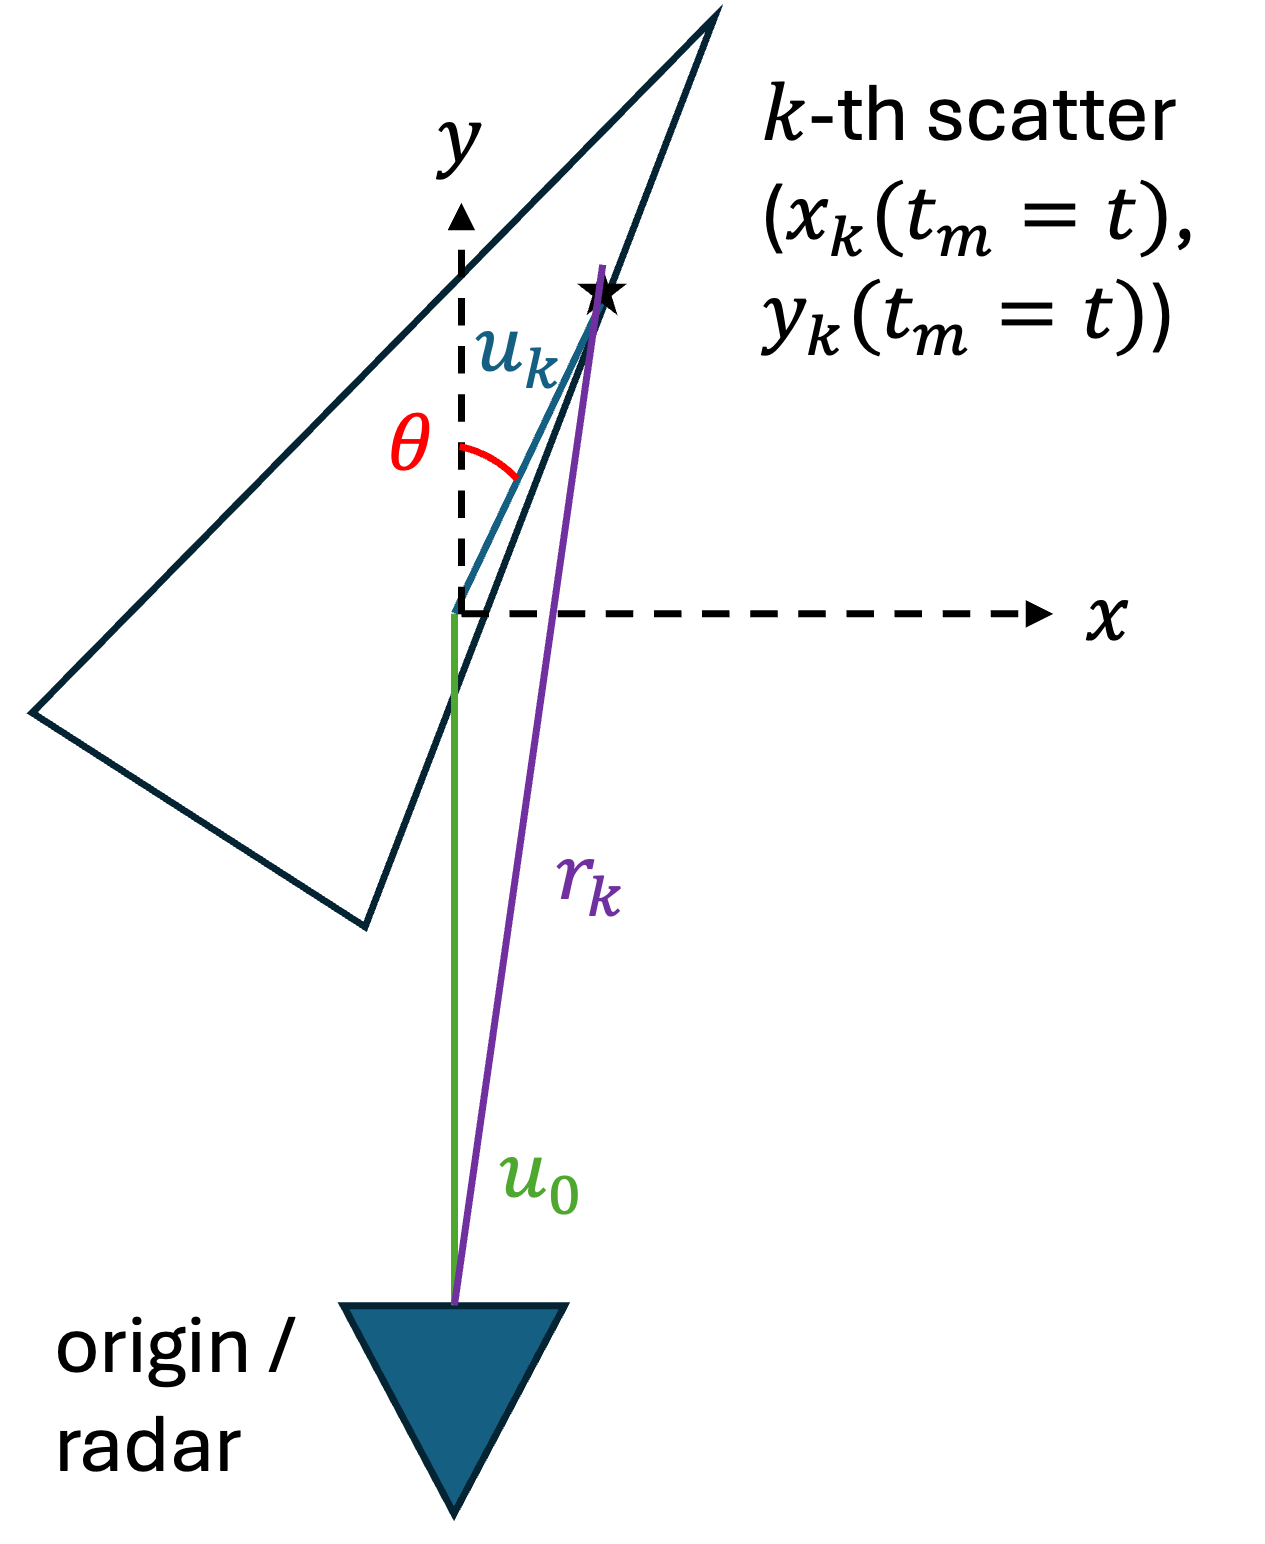
\includegraphics[width=0.3\linewidth]{isar_geo2.png}}%
    \label{fig:psf_c}
    \caption{ISAR geometry of target at (a.) $t_{m} = 0$ corresponding to the initial position of the target scatterers and (b.) at $t_{m}$ where the target has rotated $\theta(t_{m} = t) - \theta(t_{m} = 0)$}
\label{fig:geo}
\end{figure*}

\noindent The relative position of a scattering point as a function of slow-time ($t_{m}$) can be defined as \citep{Xu2022}:

\begin{equation}
    \begin{bmatrix}
        x_{k}(t_m)\\
        y_k (t_m)
    \end{bmatrix}
    =
    \begin{bmatrix}
        \cos(\theta(t_m)) & -\sin(\theta(t_{m})) \\
        \sin(\theta(t_m)) & \cos(\theta(t_m))
    \end{bmatrix}
    \begin{bmatrix}
        x_{k}\\
        y_k
    \end{bmatrix}
\end{equation}

\noindent where $\theta(t_{m})$ or $\theta_m$ is the angle of the target scatterer relative to the $y$-axis, and $[x_{k}, y_{k}]^{T}$ is the initial position of the $k$-th scatterer relative to the center of the rotation of the target. The range from the origin located at the radar to a scattering point is \citep{Xu2022}:
\begin{equation}
    \begin{aligned}
        r_{k}(t_m) &= \sqrt{x_{k}^2(t_m) + (y_k(t_{m}) + u_{0})^2}\\
        &\approx u_{0} + y_{k}(t_m) \quad \mathrm{as} \quad (y_k(t_{m}) + u_{0})^2 >> x_{k}^2(t_m)\\
        &= u_{0} + x_{k} \sin(\theta(t_{m})) + y_{k}\cos(\theta(t_{m}))\\
        &= u_{0} + u_{k} \quad \mathrm{where} \quad u_{k} = x_{k} \sin(\theta(t_{m})) + y_{k}\cos(\theta(t_{m}))
    \end{aligned} 
    \label{eq:r}
\end{equation}

\noindent The angle $\theta_m$ can be approximated using a Taylor series:

\begin{equation}
    \begin{aligned}
        \sin(\theta) &= \theta - \frac{\theta^3}{3!} + \frac{\theta^{5}}{5!} + \dots \\
        \cos(\theta) &= 1 - \frac{\theta^2}{2!} + \frac{\theta^{4}}{4!} + \dots
    \end{aligned}
\end{equation}

\noindent For most ISAR applications, the target's rotation is relatively small across the coherent integration time, enabling the usage of the small angle approximation: $\sin(\theta(t_{m})) \approx\theta(t_{m})$ and $\cos(\theta(t_m)) \approx 1$. The range from the radar to a target scatterer can be approximated as:

\begin{equation}
    r_{k}(t_{m}) \approx u_{0} + y_{k} + x_{k}\theta_{m} \quad \mathrm{where} \quad \theta(t_{m}) = \theta(0) + \omega t_{m} + \frac{\dot{\omega}}{2}t_{m}^{2} + \dots
\end{equation}


\section*{Signal model}

A linear frequency modulated (LFM) waveform is defined as:

\begin{equation}
    s(t) = \Re[\exp (j(\omega_{0}\hat{t} + \alpha \hat{t}^{2}))]
\end{equation}

\noindent where $\omega_{0}$ is the carrier wave ($\omega = 2\pi f_{c}$), $\hat{t}$ is fast-time and $\alpha$ is the chirping rate. The return chirp echo evaluated from the area of illumination, or the size of the target along the range direction from $-u_1$ to $u_1$ can be written as:

\begin{equation}
    r_{c}(\hat{t}) = A \Re \left\{ \int_{-u_{1}}^{u_{1}} g(u) \exp(j(\omega_{0}(\hat{t} - \tau_{0} - \tau(u)) + \alpha (\hat{t} - \tau_{0} - \tau(u))^{2}))du \right\}
    \label{eq:rc_t_tau}
\end{equation}

\noindent where $g(u)$ is the reflectivity of the target at $u$. The delay  $\tau_{0} = 2u_{0}/c$ is the time-delay from the radar to the center of illumination, chosen to be the center of rotation of the target, at $u_{0}$. The delay $\tau(u) = 2u/c$ is the additional delay measured from the center of the target to a point in the slant-range, $u$. In order to remove the effects of the carrier frequency, quadrature demodulation is applied. For completeness, the application is carried out in Appendix A1. The baseband continuous signal after quadrature demodulation of an LFM is \citep{Jakowatz1996}:

\begin{equation}
    \bar{r}_{c}(\hat{t}) = \frac{A}{2} \int_{-u_{1}}^{u_{1}} g(u) \exp [j[\alpha \tau^{2}(u) - \tau (u)(\omega_0 + 2\alpha (\hat{t} - \tau_{0}))]] du
    \label{eq:1.36}
\end{equation}

\noindent The nonlinear term in Equation \ref{eq:1.36} can be discarded if the target is sufficiently far away from the radar (far-field assumption) and the total illumination area, or in the case of ISAR, is the size of the target is small. Equation \ref{eq:1.36} can be simplified to:

\begin{equation}
    \begin{aligned}
        \bar{r}_{c}(\hat{t}) &= \frac{A}{2} \int_{-u_{1}}^{u_{1}} g(u) \exp [j[- \tau (u)(\omega_0 + 2\alpha (\hat{t} - \tau_{0}))]] du 
    \end{aligned}
\end{equation}

\noindent To align with typical formulations of the received echo, substitute $\omega_{0} = 2\pi f_{c}$:

\begin{equation}
    \begin{aligned}
        \bar{r}_{c}(\hat{t}) &= \frac{A}{2} \int_{-u_{1}}^{u_{1}} g(u) \exp [-j \tau (u)(2\pi f_{c} + 2\alpha (\hat{t} - \tau_{0}))] du \\
         &= \frac{A}{2} \int_{-u_{1}}^{u_{1}} g(u) \exp \left[-j \frac{4\pi u}{c}( f_{c} + f(\hat{t}))\right] du \quad \mathrm{where} \quad f(\hat{t}) = \frac{\alpha }{\pi} \hat{t} - \frac{\alpha}{\pi} \tau_{0}
    \end{aligned}
    \label{eq:ft}
\end{equation}

\noindent The last form of Equation \ref{eq:ft} contains the term $f(\hat{t})$, which is a linear change in the frequency of the return signal as a function of the fast-time. This frequency term contains the linear frequency modulation inherent to an LFM. For ISAR, there are typically a discrete, constrained number of target scatterers, allowing for Equation \ref{eq:ft} to be discretized over the target scatterers. To transition from the above formulation to defining a discrete sensing matrix, discretize the reflectivity for $K$ point scatterers located at $(u_{k} + u_{0})$.

\begin{equation}
    g(u) = \sum_{k} \sigma_{k} \delta(u - (u_{k}(t_m) + u_{0}))
    \label{eq:gu}
\end{equation}

\noindent From Equation \ref{eq:r}, the range for each scatterer is defined as a function of the rotation of the target or slow-time, necessitating the inclusion of the variable $t_{m}$ such that $\bar{r}_{c}(\hat{t}) \rightarrow \bar{r}_{c}(\hat{t},t_{m})$. Re-write Equation \ref{eq:ft} using Equation \ref{eq:gu}:

\begin{equation}
    \bar{r}_{c}(\hat{t}, t_{m}) = \frac{A}{2}\sum_{k} \sigma_{k} \exp \left[ -j \frac{4\pi (u_{k}(t_m) + u_{0})}{c} (f_{c} + f(\hat{t}))\right]
    \label{eq:rc}
\end{equation}

\noindent In order to evaluate the frequency components along the range direction, apply the FFT along the fast-time.
% why?

\begin{equation}
    r_{c}(\hat{f}, t_{m}) = \int_{-\infty}^{\infty} \frac{A}{2} \sum_{k}\sigma_{k} \exp \left[ -j \frac{4\pi (u_{k}(t_m) + u_{0})}{c} (f_{c} + f(\hat{t}))\right] \exp(j 2 \pi \hat{f}\hat{t}) d\hat{t}
    \label{eq:rc_hat_f}
\end{equation}


%\begin{equation}
%    r_{c}(\hat{t}, t_{m}) = \sum_{k} \sigma_{k} \exp{\left(-j\frac{2\pi f_{c}}{c} \tau_{k}(t_{m})\right)} \delta(\hat{t} - \tau_{k}(t_{m}))
%\end{equation}

\noindent For completeness, the application of the FFT is derived in Appendix A2. The resulting return echo after range compression is:

\begin{equation}
    \bar{r}_{c}(\hat{f}, t_{m}) = A' \sum_{k}\sigma_{k} \exp \left[ -j \frac{4\pi r_{k}(t_m)}{c} \left(f_{c}^{\text{ref}}\right)\right] \sinc ((f_{k}(t_{m})-\hat{f}) T_p)\exp \left[ -j \pi \left( f_{k}(t_{m})-\hat{f} \right)T_p\right]
    \label{eq:rc_final}
\end{equation}

\noindent Equation \ref{eq:rc} was formulated by applying quadrature demodulation and target scatterer discretization. These steps in conjunction with a FFT in fast-time combine to range compress the return echo.

\section*{Defining the linear system}

\noindent In order to leverage many of the sophisticated compressed technqiues used for image formation with suboptimal sampling, the measurement and latent image must form a linear system, $Y = AX$. The measurement ($Y$) is in the pulse $\times$ range-frequency domain. The sensing matrix ($A$) defines the physics, reflecting the return echo given the target rotation and corresponding propagation delay. The latent image $X$ is the reflectivity of the scatterers in the spatial domain, the range $\times$ crossrange domain. 

\begin{figure*}[ht]
    \centering
    \subfloat[]{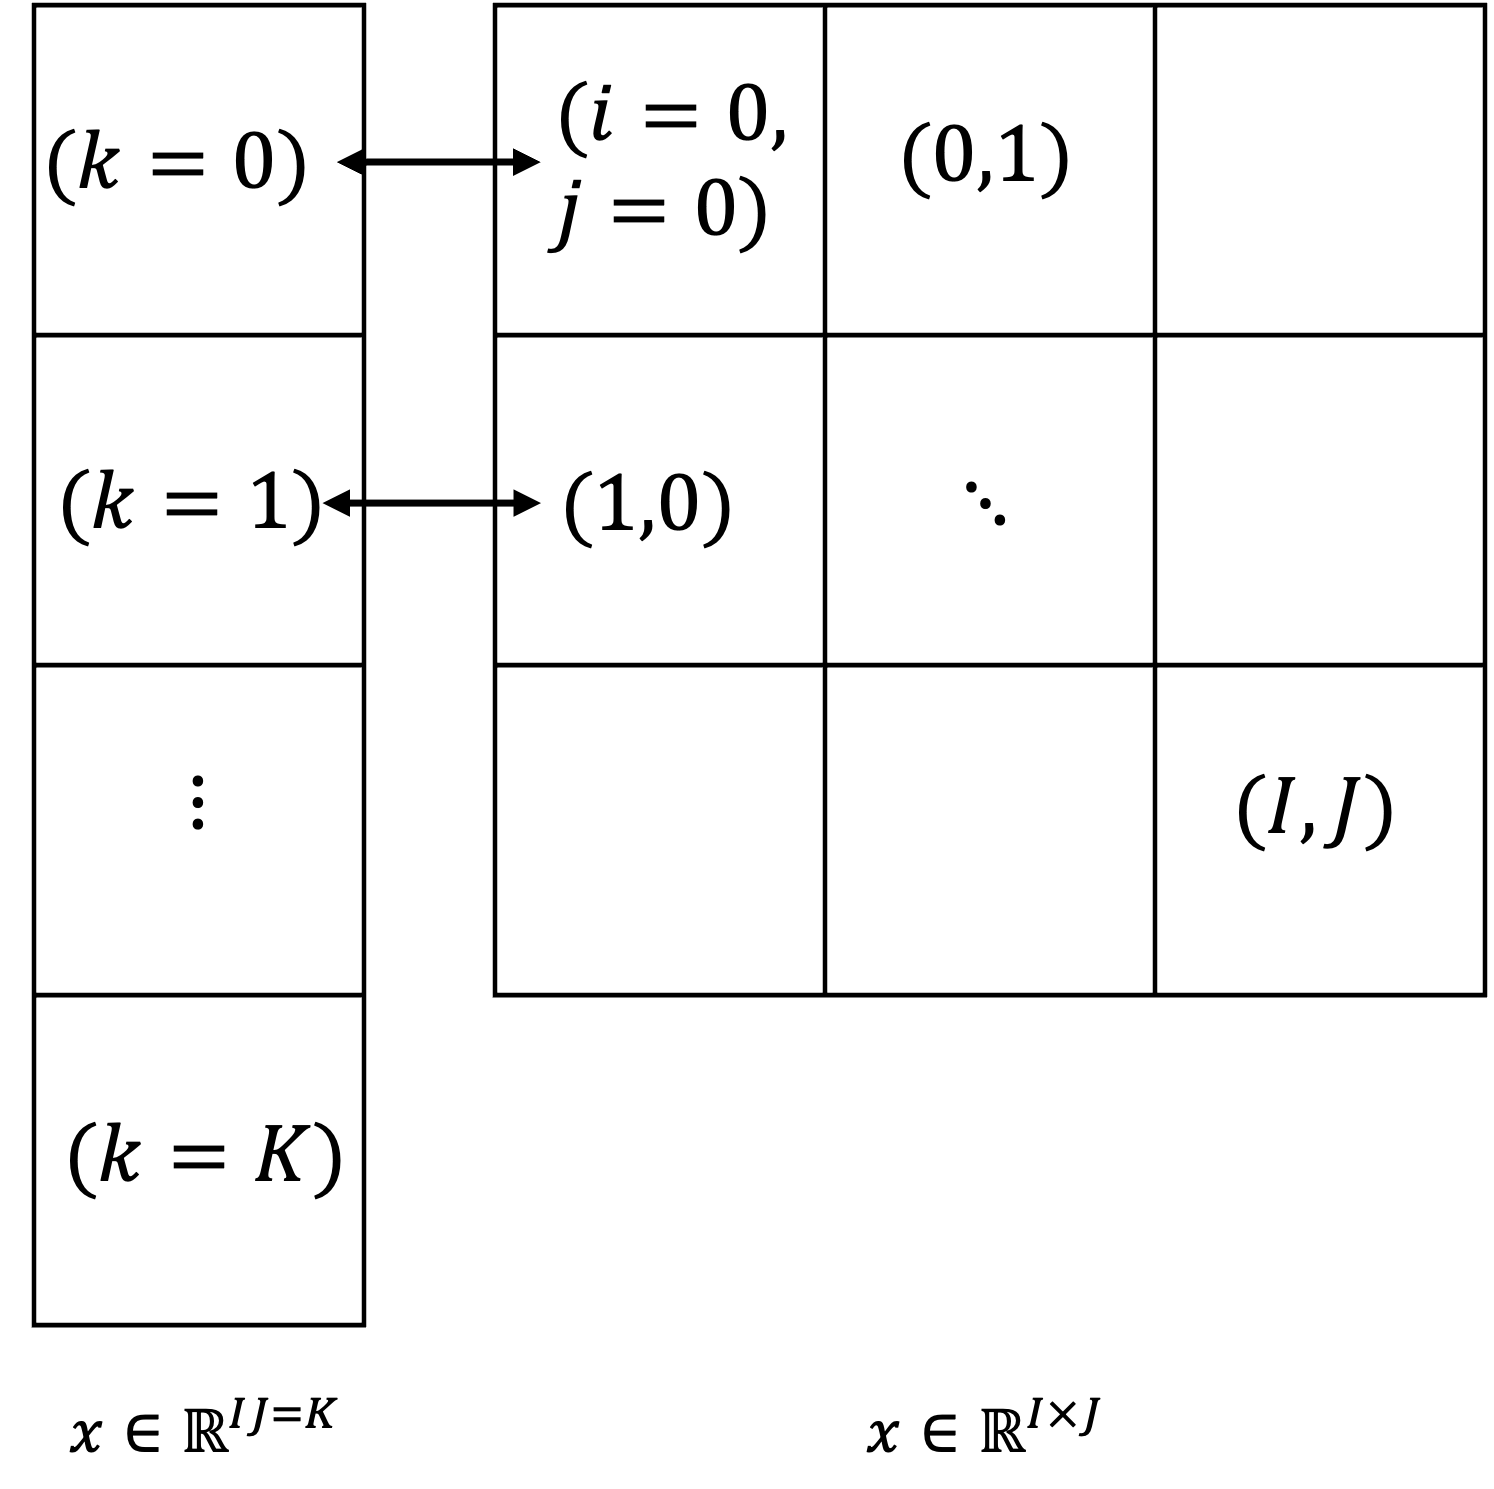
\includegraphics[width=0.3\linewidth]{range_mapping.png}}%
    \hfil
    \subfloat[]
    {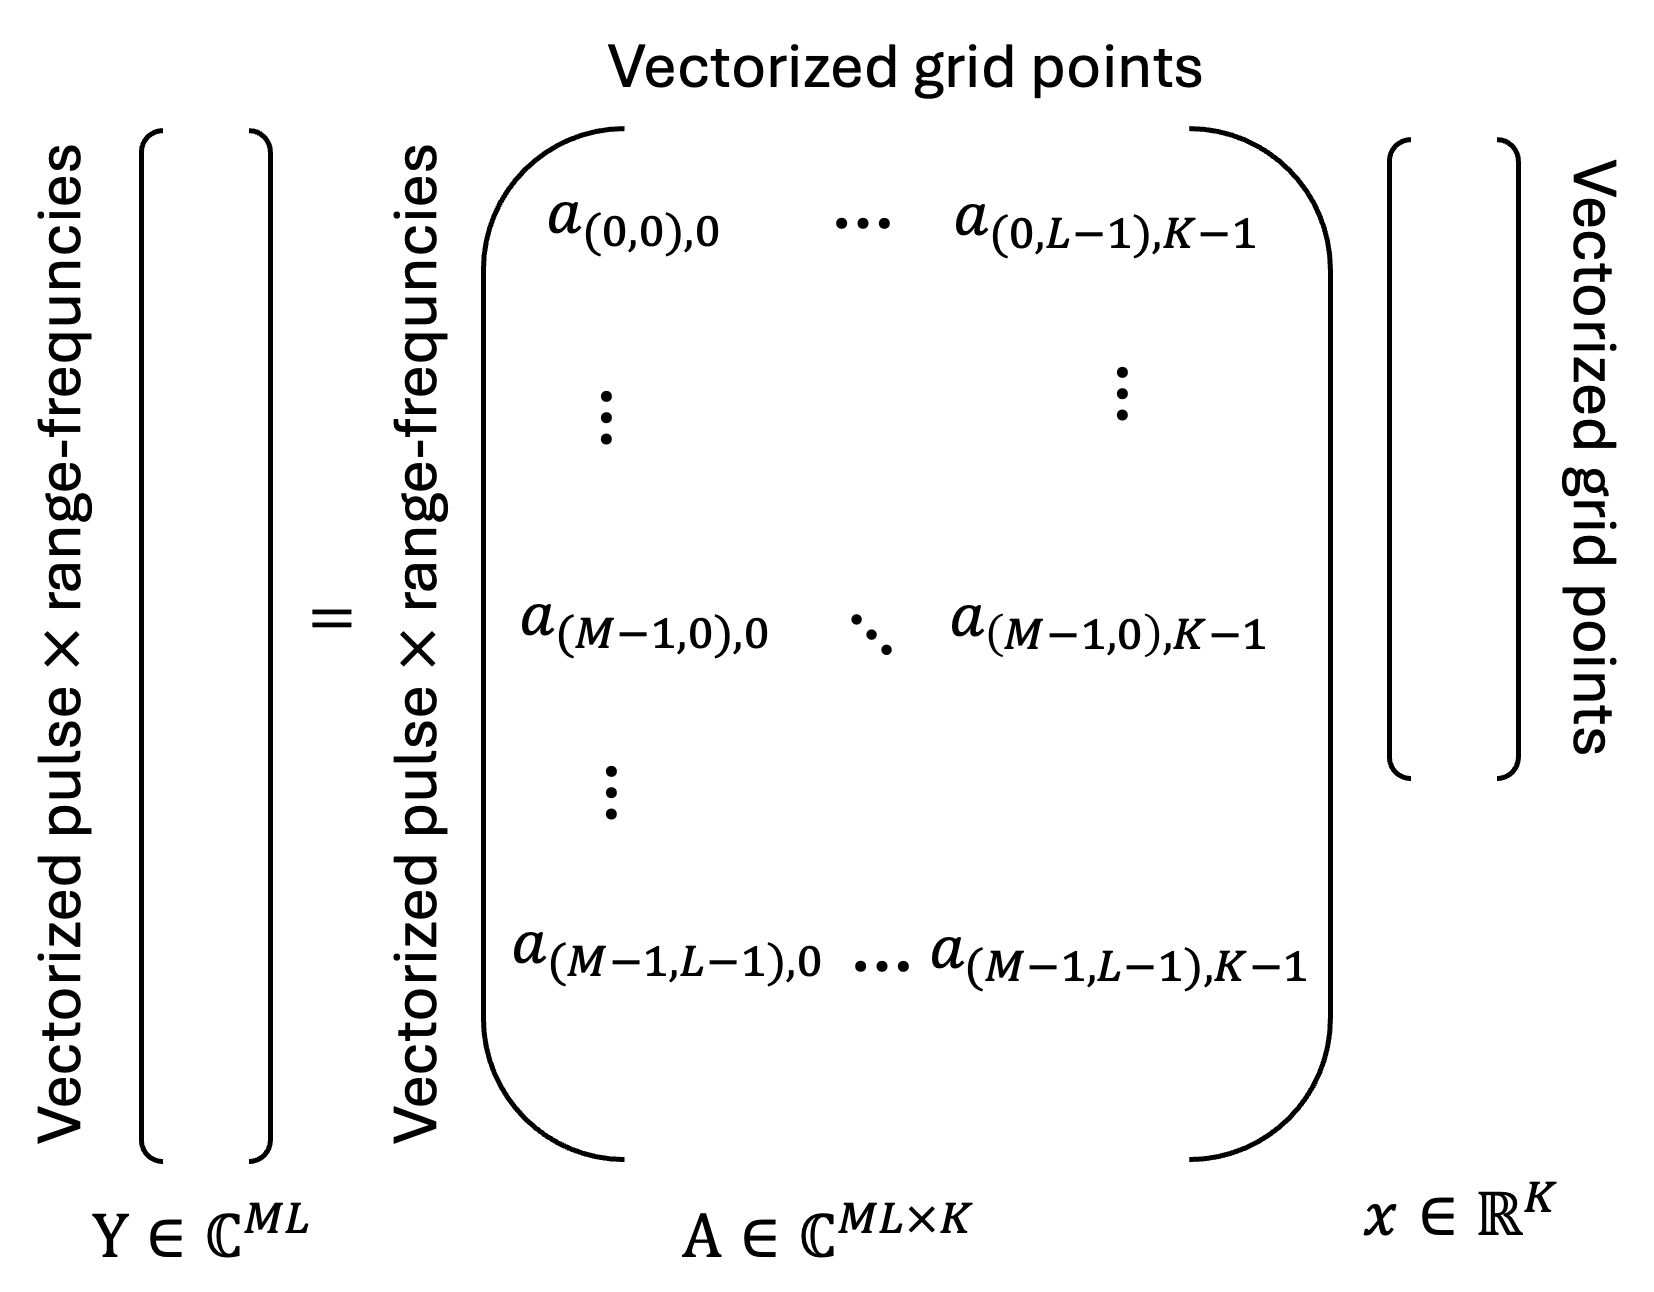
\includegraphics[width=0.5\linewidth]{linear_sys1.png}}
    \caption{ISAR linear system formulation where (a.) entries in the latent image are mapped to vector and (b.) the measurement is formed with a sensing matrix ($A \in \mathbb{C}^{ML \times K}$)}
\label{fig:lin_sys}
\end{figure*}

\noindent From Equation \ref{eq:rc_final}, the return echo is a function of each discrete target scatterer ($k$) and continuous variables, slow-time ($t_{m}$) and the range-frequency ($\hat{f}$). This equation can be reformulated, separating the reflectivity ($\sigma_{k}$) and the propagation:

\begin{equation}
    \bar{r}_{c}(\hat{f},t_{m}) = A' \sum_k \sigma_k a_k (\hat{f},t_{m})
    \label{eq:a}
\end{equation}

\noindent In order to process the entire latent image, Equation \ref{eq:a} must be scaled to include all grid points, not just those containing a target scatterer. This requires a mapping from a grid with indices $(i,j)$ to a singular index $k$. This formulation is a vectorization of the total latent image and is illustrated in Figure \ref{fig:lin_sys}. To distill the continuous variables into the sensing matrix, the slow-time and range-frequency must be discretized. The slow-time can be represented by the index $m$ where $t_{m} = m(1/\text{PRF})$ where the PRF is the pulse repetition frequency. The range-frequency can be discretized to the index $\ell$ where $\hat{f} = l(F_{s}/N)$, where $F_{s}$ is the sampling frequency and $N$ is the number of range samples. The result is a discretization of the range $r_{k}(t_{m}) \rightarrow \mathbf{r}[m,k]$, the linear variation in the frequency ($f_{k}(t_{m}) \rightarrow \mathbf{f}[m,k]$) and the range-frequency ($\mathbf{\hat{f}} \rightarrow \ell F_{s}$). Using this formulation, the entries for the sensing matrix ($A$) can be defined as:

\begin{equation}
    a[m\ell, k] = \exp \left[ -j \frac{4\pi f_{c}^{\text{ref}}}{c} \mathbf{r}[m,k] \right] \sinc (\mathbf{f}[m,k]-\mathbf{\hat{f}}[\ell]) T_p)\exp \left[ -j \pi \left( \mathbf{f}[m,k]-\mathbf{\hat{f}}[\ell] \right))T_p\right]
\end{equation}

\bibliography{sample}

\section*{Appendix}

\subsection*{A1: Quadrature demodulation derivation}

Apply in-phase and quadrature mixing using scaled and delayed versions of the LFM chirp \citep{Jakowatz1996}:

\begin{equation}
    \begin{aligned}
        c_{I}(\hat{t}) &= \cos(\omega_{0}(\hat{t} - \tau(u)) +\alpha(\hat{t} - \tau(u))^{2}) \\
        c_{Q}(\hat{t}) &= \sin(\omega_{0}(\hat{t} - \tau(u)) +\alpha(\hat{t} - \tau(u))^{2})
    \end{aligned}
    \label{eq:IQ}
\end{equation}

\noindent To mix, multiply Equation \ref{eq:rc_t_tau} by both terms in Equation \ref{eq:IQ}. Starting with the in-phase term:

\begin{equation}
    \begin{aligned}
        r_{I}(\hat{t}) &= A   \int_{-u_{1}}^{u_{1}} \Re \left\{ g(u) \exp(j(\omega_{0}(\hat{t} - \tau_{0} - \tau(u)) + \alpha (\hat{t} - \tau_{0} - \tau(u))^{2})) \right\} \cos(\omega_{0}(\hat{t} - \tau(u)) +\alpha(\hat{t} - \tau(u))^{2}) du  \\
        &= A   \int_{-u_{1}}^{u_{1}} g(u) \cos(\omega_{0}(\hat{t} - \tau_{0} - \tau(u)) + \alpha (\hat{t} - \tau_{0} - \tau(u))^{2} ) \cos(\omega_{0}(\hat{t} - \tau(u)) +\alpha(\hat{t} - \tau(u))^{2}) du
    \end{aligned}
\end{equation}

\noindent Use the identity: $\cos(A)\cos(B) = 1/2[\cos(A-B) + \cos(A+B)]$:

\begin{equation}
    \begin{aligned}
        r_{I}(\hat{t}) 
        =& \frac{A}{2} \int_{-u_{1}}^{u_{1}} g(u) \cos(\omega_{0}(\hat{t} - \tau_{0} - \tau(u)) + \alpha (\hat{t} - \tau_{0} - \tau(u))^{2} -\omega_{0}(\hat{t} - \tau(u)) -\alpha(\hat{t} - \tau(u))^{2}) du\\
        +&\frac{A}{2} \int_{-u_{1}}^{u_{1}} g(u) \cos(\omega_{0}(\hat{t} - \tau_{0} - \tau(u)) + \alpha (\hat{t} - \tau_{0} - \tau(u))^{2} +\omega_{0}(\hat{t} - \tau(u)) +\alpha(\hat{t} - \tau(u))^{2}) du
    \end{aligned}
    \label{eq:quad1}
\end{equation}

\noindent Expanding the roots, $(\hat{t} - \tau_{0} - \tau(u))^{2} = \hat{t}^2 -2\hat{t}\tau_{0} - 2\hat{t}\tau(u) + 2\tau_{0}\tau(u) + \tau_{0}^{2} + \tau(u)^{2}$ and $(\hat{t} - \tau(u))^{2} = \hat{t}^{2} - 2\hat{t}\tau(u) + \tau(u)^{2}$ and combining like terms reduces Equation \ref{eq:quad1}:

\begin{equation}
    \begin{aligned}
        r_{I}(\hat{t}) 
        =& \frac{A}{2} \int_{-u_{1}}^{u_{1}} g(u) \cos(-\omega_{0}\tau(u) - 2\alpha \hat{t}\tau(u) + 2\alpha \tau_{0}\tau(u) + \alpha\tau(u)^{2}) du\\
        +&\frac{A}{2} \int_{-u_{1}}^{u_{1}} g(u) \cos(2\omega\hat{t} - 2\omega_{0}\tau_{0} - \omega_{0}\tau(u) + 2\alpha\hat{t}^{2} - 4\alpha\hat{t}\tau_{0} - 2\alpha\hat{t}\tau(u) \\
        +& +2\alpha\tau_{0}^2 + 2\alpha\tau_{0}\tau(u) + \alpha\tau(u)^{2} )du\\
        =& \frac{A}{2} \int_{-u_{1}}^{u_{1}} g(u) \cos(\alpha\tau(u)^{2} - \tau(u)(\omega_{0} + 2\alpha(\hat{t} - \tau_{0}))) du\\
        +&\frac{A}{2} \int_{-u_{1}}^{u_{1}} g(u) \cos(\omega_{0}(2\hat{t} - \tau(u) - 2\tau_{0}) + \alpha((\hat{t} - \tau_{0})^{2} + (\hat{t} - \tau(u) - \tau_{0})^{2})du
    \end{aligned}
    \label{eq:quad1}
\end{equation}

\noindent The second term in $r_{I}(\hat{t})$ has a center frequency term of $2\omega_{0}$ which is filtered out after applying a low-pass filter. The remaining in-phase term is:

\begin{equation}
    r_{I}(\hat{t}) = \frac{A}{2} \int_{-u_{1}}^{u_{1}} g(u) \cos(\alpha\tau(u)^{2} - \tau(u)(\omega_{0} + 2\alpha(\hat{t} - \tau_{0}))) du
\end{equation}

\noindent Using the same derivation methodology and low-pass filtering, the quadrature term can be determined as \citep{Jakowatz1996}:

\begin{equation}
    r_{I}(\hat{t}) = \frac{A}{2} \int_{-u_{1}}^{u_{1}} g(u) \sin(\alpha\tau(u)^{2} - \tau(u)(\omega_{0} + 2\alpha(\hat{t} - \tau_{0}))) du
\end{equation}

\noindent The quadrature demodulated signal can therefore be written as:

\begin{equation}
    r_{I}(\hat{t}) = \frac{A}{2} \int_{-u_{1}}^{u_{1}} g(u) \exp(-j(\alpha\tau(u)^{2} - \tau(u)(\omega_{0} + 2\alpha(\hat{t} - \tau_{0})))) du
\end{equation}


\subsection*{A2: FFT of return echo and verification}\label{ap:fft}
From Equation \ref{eq:rc_hat_f}, isolate the terms explicitly dependent on the fast-time, $\hat{t}$, and move the other terms on the left-hand side of the integral:

\begin{equation}
\begin{aligned}
    r_{c}(\hat{f}, t_{m}) &= \int_{-\infty}^{\infty} \frac{A}{2} \sum_{k}\sigma_{k} \exp \left[ -j \frac{4\pi (u_{k}(t_m) + u_{0})}{c} f_{c}\right]
    \exp \left[ -j \frac{4\pi (u_{k}(t_m) + u_{0})}{c} f(\hat{t})\right]
    \exp(j 2 \pi \hat{f}\hat{t}) d\hat{t} \\
    &= \frac{A}{2} \sum_{k}\sigma_{k} \exp \left[ -j \frac{4\pi (u_{k}(t_m) + u_{0})}{c} f_{c}\right]\int_{-\infty}^{\infty} 
    \exp \left[ -j \frac{4\pi (u_{k}(t_m) + u_{0})}{c} f(\hat{t})\right]
    \exp(j 2 \pi \hat{f}\hat{t}) d\hat{t}
\end{aligned}
\end{equation}

\noindent For clarity's sake and notational ease substitute $r_{k}(t_{m}) = u_{0} + u_{k}(t_{m})$:

\begin{equation}
\begin{aligned}
    r_{c}(\hat{f}, t_{m})
    &= \frac{A}{2} \sum_{k}\sigma_{k} \exp \left[ -j \frac{4\pi r_{k}(t_m)}{c} f_{c}\right]\int_{-\infty}^{\infty} 
    \exp \left[ -j \frac{4\pi r_{k}(t_{m})}{c} f(\hat{t})\right]
    \exp(j 2 \pi \hat{f}\hat{t}) d\hat{t}
\end{aligned}
\label{eq:fft1}
\end{equation}

\noindent Define the portion of Equation \ref{eq:fft1} containing the integral as:
\begin{equation}
    \begin{aligned}
        I(\hat{f}, t_{m})
        &= \int_{-\infty}^{\infty} 
        \exp \left[ -j \frac{4\pi r_{k}(t_{m})}{c} f(\hat{t})\right]
        \exp(j 2 \pi \hat{f}\hat{t}) d\hat{t}\\
        &= \int_{-\infty}^{\infty} 
        \exp \left[ -j 2\pi \left( \frac{2 r_{k}(t_{m})}{c} f(\hat{t}) - \hat{f}\hat{t} \right)\right]
         d\hat{t}
    \end{aligned}
    \label{eq:fft2}
\end{equation}

\noindent From Equation \ref{eq:1.36} and \ref{eq:ft}, the linearly increasing frequency component of the LFM is defined as $f(\hat{t}) = (\alpha/\pi) \hat{t} - (\alpha/\pi) \tau_{0}$. Substituting $f(\hat{t})$ into Equation \ref{eq:fft2}, and moving the portion of the integrand not explicitly dependent on the fast-time to the left-hand side of the integral:

\begin{equation}
    \begin{aligned}
        I(\hat{f}, t_{m})
        &= \int_{-\infty}^{\infty} 
        \exp \left[ -j 2\pi \left( \frac{2 r_{k}(t_{m})}{c} \left( \frac{\alpha}{\pi} \hat{t} - \frac{\alpha}{\pi}\tau_{0} \right) - \hat{f}\hat{t} \right)\right]
         d\hat{t}\\
         &= \int_{-\infty}^{\infty} 
        \exp \left[ -j 2\pi \left( \frac{2 r_{k}(t_{m})}{c} \left( \frac{\alpha}{\pi} \right) - \hat{f} \right)\hat{t}\right]
        \exp \left[ -j 2\pi \left( \frac{2 r_{k}(t_{m})}{c} \left( - \frac{\alpha}{\pi}\tau_{0} \right) \right)\right]
         d\hat{t}\\
         &= \exp \left[ -j 2\pi \left( \frac{2 r_{k}(t_{m})}{c} \left( - \frac{\alpha}{\pi}\tau_{0} \right) \right)\right] \int_{-\infty}^{\infty} 
        \exp \left[ -j 2\pi \left( \frac{2 r_{k}(t_{m})}{c} \left( \frac{\alpha}{\pi} \right) - \hat{f} \right)\hat{t}\right]
         d\hat{t}
    \end{aligned}
    \label{eq:fft3}
\end{equation}

\noindent Because the radar will only process the fast-time over the interval of a pulse duration, modify the bounds to $0$ to $T_{p}$. Define the portion of Equation \ref{eq:fft3} within the integral and solve the integral:

\begin{equation}
    \begin{aligned}
        I'(\hat{f}, t_{m})
         &= \int_{0}^{T_{p}} 
        \exp \left[ -j 2\pi \left( f_{k}(t_{m}) - \hat{f} \right)\hat{t}\right]
         d\hat{t} \quad \mathrm{where} \quad f_{k}(t_{m}) = \left( \frac{2 r_{k}(t_{m})}{c} \right) \left(\frac{\alpha}{\pi}\right)\\
         &= \int_{0}^{T_{p}} 
        \exp \left[ -j 2\pi \Delta f \hat{t}\right]
         d\hat{t} \quad \mathrm{where} \quad \Delta f = f_{k}(t_{m}) - \hat{f}\\
         &= \frac{\exp \left[ -j 2\pi \left( \Delta f \right)\hat{t}\right]}{-j 2\pi \left( \Delta f \right)} \bigg\rvert_{0}^{T_p}\\
         &= \frac{\exp \left[ -j 2\pi \left( \Delta f \right)T_p\right] - 1}{-j 2\pi \left( \Delta f \right)}
    \end{aligned}
    \label{eq:fft4}
\end{equation}

\noindent In order to simplify Equation \ref{eq:fft4} to a more familiar form, use the identity: \\$\exp(-j\theta)-1 = \exp(-j\theta/2)(\exp(-j\theta/2) - \exp(+j\theta/2))$:

\begin{equation}
    \begin{aligned}
        I'(\hat{f}, t_{m})
         &= \frac{\exp \left[ -j \pi \left( \Delta f \right)T_p\right]\left( \exp \left[ -j \pi \left( \Delta f \right)T_p\right] - \exp \left[ j \pi \left( \Delta f \right)T_p\right] \right)}{-j 2\pi \left( \Delta f \right)} \\
         &= \frac{\exp \left[ -j \pi \left( \Delta f \right)T_p\right]\left( -2j\sin(\pi \left( \Delta f \right)T_p) \right)}{-j 2\pi \left( \Delta f \right)} \quad \mathrm{as} \quad \sin(\theta) = \frac{\exp(j\theta) - \exp{(-j\theta)}}{2j} \\
         &= \frac{\sin(\pi \left( \Delta f \right)T_p) }{\left(\pi \Delta f \right)}\exp \left[ -j \pi \left( \Delta f \right)T_p\right]\\
         &= T_p \sinc (\Delta f T_p)\exp \left[ -j \pi \left( \Delta f \right)T_p\right]
    \end{aligned}
    \label{eq:fft5}
\end{equation}

\noindent Recombine terms to form the final return echo in the pulse by range-frequency domain:
\begin{equation}
    \begin{aligned}
        \bar{r}_{c}(\hat{f},T_{m}) =& \frac{A}{2} \sum_{k}\sigma_{k} \exp \left[ -j \frac{4\pi r_{k}(t_m)}{c} f_{c}\right] \exp \left[ -j 2\pi \left( \frac{2 r_{k}(t_{m})}{c} \left( - \frac{\alpha}{\pi}\tau_{0} \right) \right)\right]\\ 
        &T_p \sinc ((f_{k}(t_{m})-\hat{f}) T_p)\exp \left[ -j \pi \left( (f_{k}(t_{m})-\hat{f} \right)T_p\right] \\
        =& \frac{A}{2} \sum_{k}\sigma_{k} \exp \left[ -j \frac{4\pi r_{k}(t_m)}{c} \left(f_{c}  - \frac{\alpha}{\pi}\tau_{0} \right)\right] 
        T_p \sinc ((f_{k}(t_{m})-\hat{f}) T_p)\exp \left[ -j \pi \left( (f_{k}(t_{m})-\hat{f} \right)T_p\right]\\
        =& \frac{A}{2} \sum_{k}\sigma_{k} \exp \left[ -j \frac{4\pi r_{k}(t_m)}{c} \left(f_{c}^{\text{ref}}\right)\right] 
        T_p \sinc ((f_{k}(t_{m})-\hat{f}) T_p)\exp \left[ -j \pi \left( (f_{k}(t_{m})-\hat{f} \right)T_p\right]
    \end{aligned}
    \label{eq:fft_final}
\end{equation}

\noindent where the scaling factor $A$ has absorbed the pulse duration and additional factor of $1/2$, $A' = AT_p/2$. From Equation \ref{eq:fft_final}, $f_{c}^{\text{ref}}$ can be thought of as the center frequency referenced at a chosen fast-time origin $\tau_{0} = 2R_{0}/c$. To validate Equation \ref{eq:fft_final}, compare this formulation to the simplified version typically defined in literature, where the target scatterers are assumed to be on-grid. If the target scatterers are on-grid, $f_{k}(t_{m}) = \hat{f}$ and $\sinc ((f_{k}(t_{m})-\hat{f}) T_p) = \sinc (0) = 1$ and $\exp \left[ -j \pi \left( (f_{k}(t_{m})-\hat{f} \right)T_p\right] = \exp \left[ -j \pi \left( (0 \right)T_p\right] = 1$. The final result of collapsing the range-frequencies $\hat{f}$ into the bins defined by $f_{k}(t_{m})$ is:

\begin{equation}
    \bar{r}_{c}(\hat{f}, t_{m}) = A' \sum_{k}\sigma_{k} \exp \left[ -j \frac{4\pi r_{k}(t_m)}{c} \left(f_{c}^{\text{ref}}\right)\right] 
    \label{eq:fft_verf}
\end{equation}

\noindent Equation \ref{eq:fft_verf} coincides with the typical formulation of the range-compressed LFM where the scatterers are approximated as on-grid. Thus concludes the derivation of the FFT of the return baseband LFM.

\end{document}